\section{Селективное лазерное спекание}

\begin{figure}[h]
    \centering
    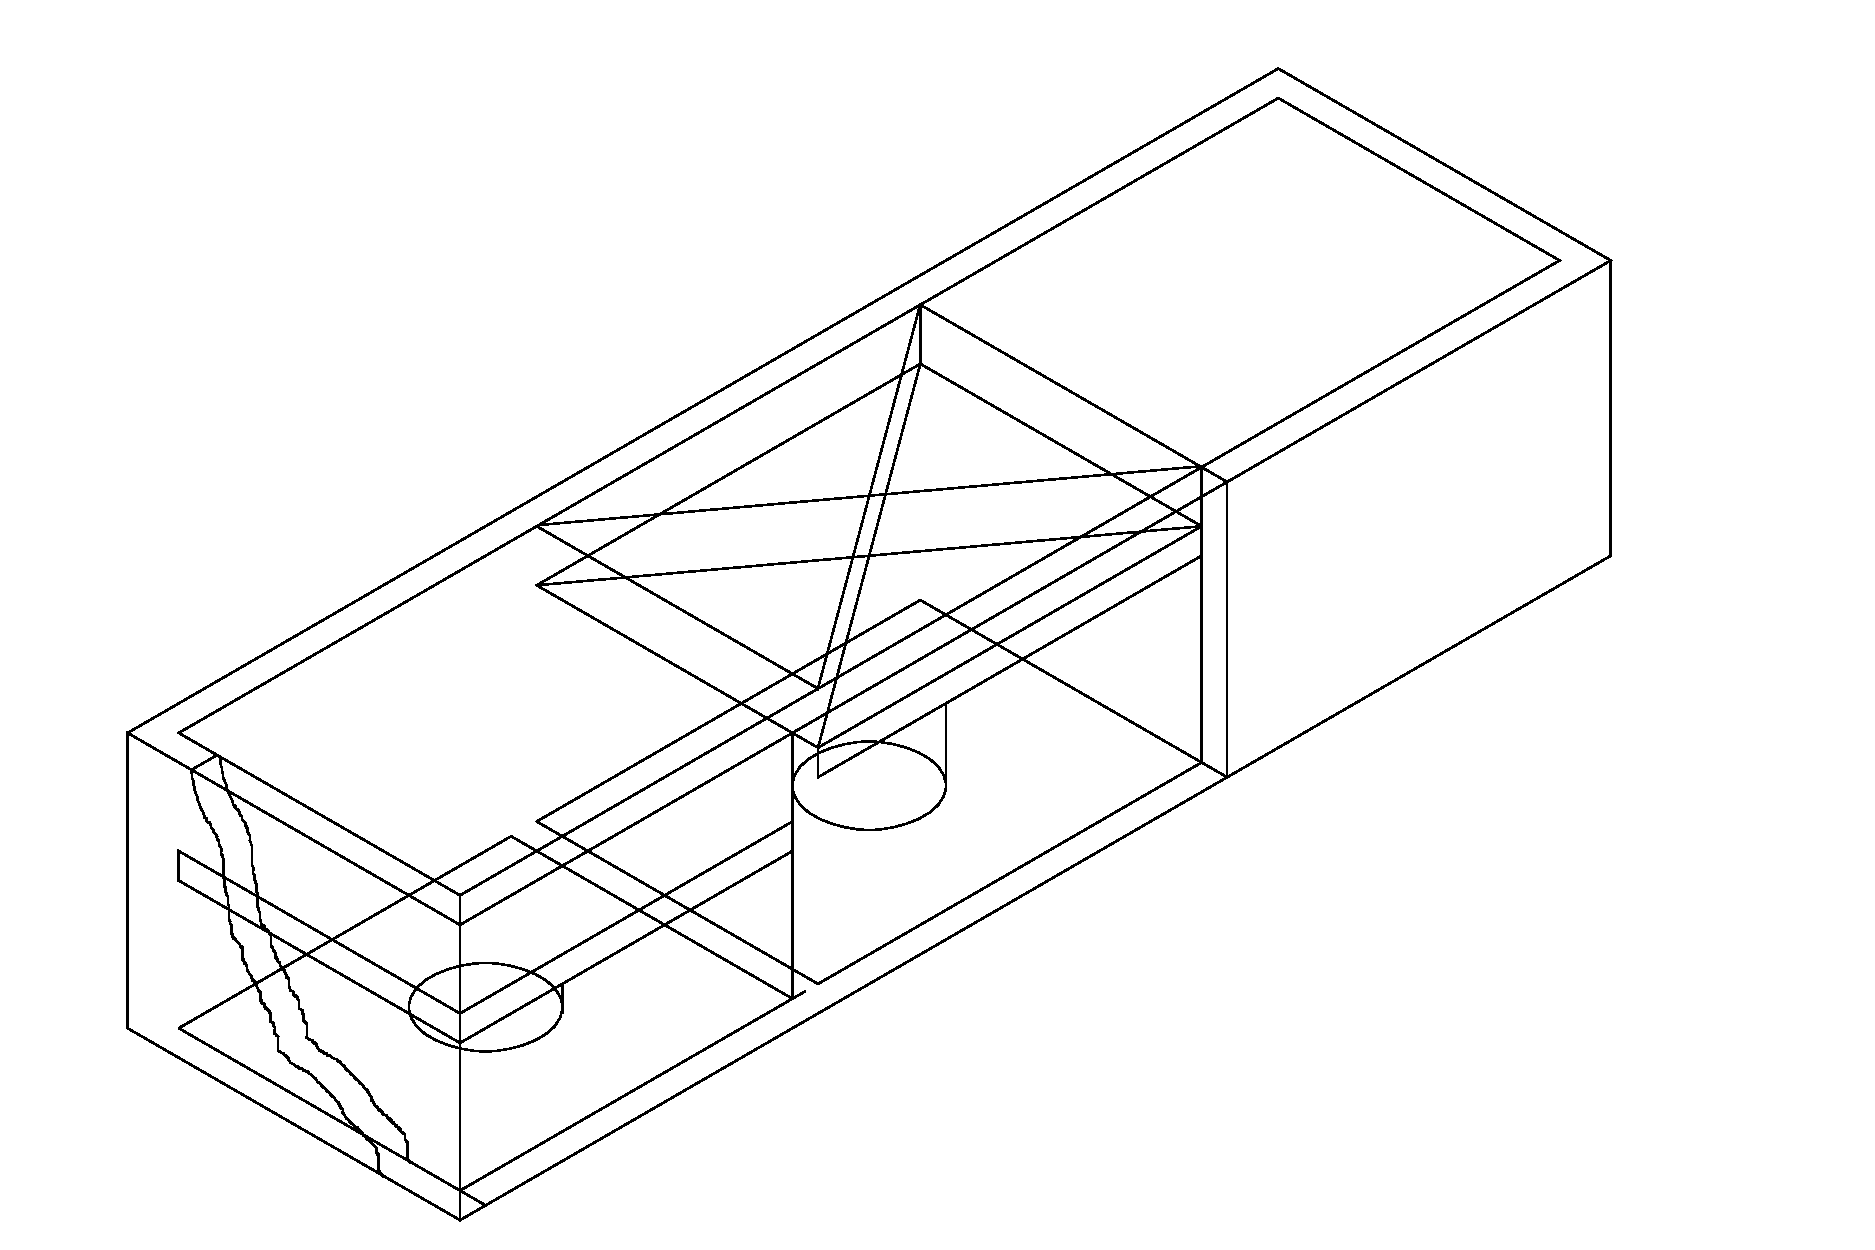
\includegraphics[width=\linewidth]{fig/sls-30deg.pdf}
    \caption{[WIP]Принцип работы SLS-принтера}
    \label{fig:printer}
\end{figure}

\paragraph{Что это вообще}
\paragraph{Общий принцип. }Процесс печати изделия изображен схематически на рис. \ref{fig:printer}.
\paragraph{Особенности сравнению с традиционными методами.}
\paragraph{Особенности по сравнению с другой 3д-печатью.}
\paragraph{Симуляция процесса close-up.}


% вся инфа которая пока есть
Высокая интенсивнсть лазерного излучения позволяет быстро нагревать небольшие участки материала, создавая большие градиенты температур \cite{sls-sim2016}.
\\
Симуляция СЛС показывает, что у композитных порошков будет сильно отличное распределение температур, особенно глубина плавления. (по крайне мере в полиамидах)\cite{sls-sim2016}. Экспериментальное исследование становится эфеективнее, если есть модель процесса.
Какие нужны параметры для модели?
%%%%%%%%%%%%%%%%%%%%%%%%%%%%%%%%%%%%%%%%%%%%%%

\section{Требования к материалам для СЛС}

%вступление
Конечные характеристики изделия, полученного по технологии СЛС, во многом зависят от от свойств начального порошка (морфология, размер, распределние размеров, объемная плотность, термические свойства, вязкость, поверхностное натяжение )  и параметров спекания (мощность лазера, скорость сканирования, диаметр пятна излучения лазера ).

\subsection{Механические характеристики}
первая глава из
\cite{termopols}
\subsection{Тепловые характеристики}
\subsection{Морфология частиц порошка}
Морфология частиц определяет пространственное расположение частиц порошка (stacking degree) относительно друг друга. Сферические (с гладкой поверхностью) частицы имеют высокую плотность упаковки. Они обеспечивают  сыпучесть in systems of applying the material with minimal resistance. В добавок, сферические частицы хорошо связываются в процессе спекания.Показано, что 
during the transition from powder particles with predominantly spherical morphology to particles of irregular shape of the same material, the elastic modulus decreases by almost 40 \%. 
(найти ссылку ,потом перевести).
Таким образом, сферический частицы с хорошей сыпучестью и высокой плотностью упаковки представляют идеальные характеристики стартового пороша для испольщования в СЛС.\\
В то же время использование частиц неправильной формы с большой вариацией в размерах ведет к созданию продуктов с более высокими механическими характеристиками в сравнении с использованием mainle сферических частиц с узким распределением размеров.

\subsection{Кристалличность}

\subsection{Прочее}


\subsection{Полиэфиримиды ряда R-BAPB }
		
	\begin{figure}[h]
	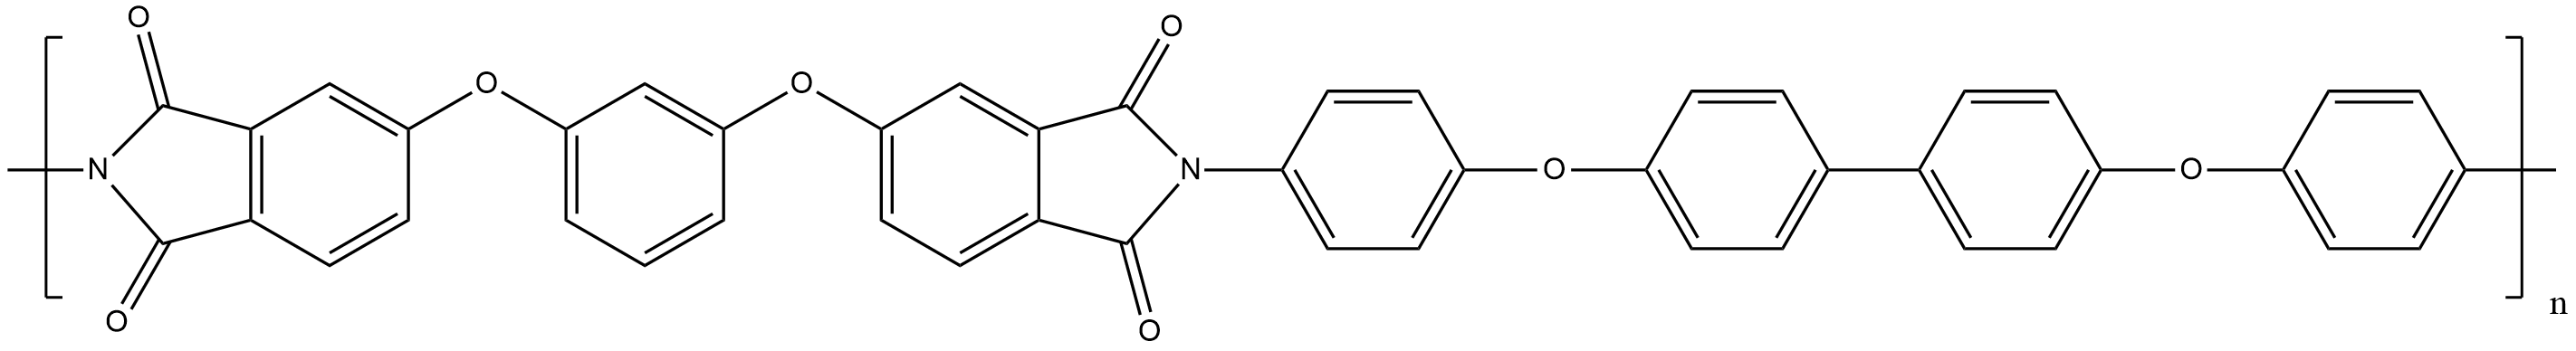
\includegraphics[width=\textwidth]{fig/formula.png}
	\caption{Структура полимера Р-ОДФО \cite{pi-formula}}
	\label{fig:formula}
	\end{figure}

Что это\\
Особенности\\
Намеренные ранее характеристики\\
Использование в промышленности\\
Композиты\\
Короче, они збс и подходят для СЛС\\
Что нужно выяснить.\\

\section{Кристаллическая структура полимеров}

Что ее характеризует
Поскольку кристаллические области в этих полимерах формируются из длинных цепей, их кристаллизация сложна и сильно чувствительа к маленьким изменениям в полимерной (compostion), добавкам, температуре и механическим воздействиям.\\
Не все полимеры кристаллизуются, а те, что кристаллизуются, редко делают это полностью: только небольшая часть crystallizable цепей incorporated into crystalline domains, а остальные segregate into amorphous domains. Степеь кристалличности и характеристики кристаллических domains являются самыми важными морфологическими характеристиками, которые определяют физические свойства такие как плотность, mechanical strength, processability, permeability and degradability частичнокристаллического полимера.\\
Степень кристалличности типичного полимера варьируется в пределах от 10 до 80 \%. Сравните с металлами, которые, за исключением металлических стекол, почти всегда полностью кристалличны, и ceramics, которые или полностью кристалличны, или аморфны.\\ \cite{cryst3} или \cite{cryst1}






Кристаллическая структура полимеров менее идеальна чем кристаллы соединений с меньшей молекулярной массой. Как правило полимерные материалы находятся в метастабильном состоянии, то есть являются частично кристаллическими и частично аморфными. Большинсво полимеров частичнокристалличны по структуре, кристаллические структуры часто формируются при охлаждении расплава, что контролирует механические и физические свойства частичнокристаллических полимеров. Ввиду высокой вязкости полимерных расплавов, полимеры кристаллизуются очень медленно при температурах ниже температуры плавления ($T_m$), даже при высоком переохлаждении (high supercooling)
\\
Кристаллическая структура и степень кристалличости зависят от молекулярной структуры полимера, условий (growth
conditions), присутствия инородых частиц в решетке, температуры кристаллизации, скорости охлаждения и т.д.\\
Они могут быть оценены из рентгеновской дифракции, измерений плотности, термического аналища и т.д.

\subsection{Кристаллиты}
Морфологии полимерных кристаллов можно условно поделить на ламеллярные и фибриллярные кристаллы. В процессе ламеллярной кристаллизации, направление роста перпендикулярно направлению цепи, возникает складываение цепочки.Во время фибриллярной кристаллизации, наплавление роста кристалла совпадает с направление цепи, и в решетке кристалла возникают highly extended chain conformations. Такие материалы имеют высокие механические свойства. Кристаллизация существенно меняет физические и механические свойства полимерных систем. \\

Studying the crystallization
behavior, though complicated, is necessary mainly in relation to the physical and
mechanical properties of polymers. If crystallization would be absent in polymer
systems, then the whole mechanical performance of polymers depends on the glass
transition temperature (Tg). If glass transition is the only determining factor for the
properties of the polymers, then polymers such as polypropylene (PP) and PE
would have been rubbers at ambient temperature. However, in these polymers,
due to crystallization, the stiffness is retained at acceptable and controllable values
up to the melting temperature (Tm).\\
Multiphase polymer systems commonly consist of polymer blends, composites,
nanocomposites, interpenetrating polymer networks, block copolymers, and polymer
gels. Crystallization in multicomponent polymer-based systems represents the main
physical characteristic that allows for control of the material properties.\\
The presence of nanoparticles
can also limit themotion ofmolecular chains, resulting in suppression of the crystalline
perfection and crystallinity of polymer crystals.\\
Crystallization is a first-order transition and a thermal process in polymers. The
polymer chains are aligned and folded together to form an ordered chain region,
which is called lamellae. The lamellae are composed of spherical aggregates called
spherulites. The crystallization process changes the density, symmetry, and phase
transition and thus controls the properties of the end products. Crystallization
commonly proceeds by nucleation of a fiberlike structure followed by lamellar
structure formation. The spherulites grow away from a nucleation site.\\
Nowadays polymer composites are commonly used in aerospace, sport goods, automobiles,
industrial equipment, etc. Polymer composites are polymer-based matrix
with some form of materials embedded in the matrix, as reinforcements.\\
Polymer composites are classified on the basis of the size of filler particles into
microcomposites and nanocomposites.\\
(Это в планы на будущее)
Many experimental techniques can be used to study the crystallization
kinetics of nanocomposites. The most common techniques used to study the
crystallization kinetics in the nanocomposites are DSC, optical microscopy, and
WAXD.\\
The crystallization
kinetics of polymer composites and nanocomposites gained great interest due to the
fact that fillers act as an effective nucleating agent in the polymer matrix. With the
advancement of nanotechnology, the focus is now shifting toward understanding
the crystallization properties of materials in nanodimensions and thereby tune the
properties for diversified tailored application.\\

Это все из \cite{cryst1}

	\begin{wrapfigure}{r}{0.5\textwidth} 
\vspace{-20pt}


  \begin{center}
    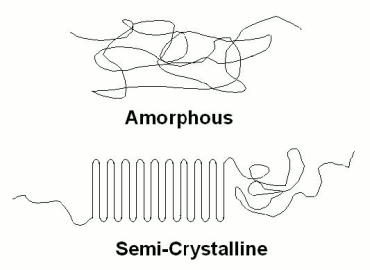
\includegraphics[width=0.4\textwidth]{fig/crystal-1.png}
    \caption{Как цепочки складываются в ламели}
    \label{fig:crystal-1}
  \end{center}
  \vspace{-20pt}
  \vspace{1pt}
\end{wrapfigure}



\begin{figure}[h]
    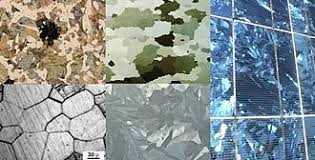
\includegraphics[width=\textwidth]{fig/crystallites.jpg}
    \caption{Типы кристаллитов}
    \label{fig:crystallites}
\end{figure}



\subsection{Частичная кристалличность}
Properties of the semicrystalline polymers can be understood, for the most part,
using a simple two-phase model that assumes that the two phases, the crystalline and
the amorphous, can be easily distinguished. If an intensive property $\phi$ (e.g., specific
volume, specific heat) of the crystalline and amorphous phases, $\phi$ c and $\phi$a, respectively, can be measured, and if we assume that contributions of the two phases
are additive, then
\[ 
\phi = \phi_c x + \phi_a(1-x)
\]
where x is the fraction of the crystalline phase, which ideally is the mass fraction
(x\_m) but depends somewhat on the technique (это из \cite{cryst3})
The
smallest organized units of polymer chains are crystallites or lamellae. These further
assemble to form fibrils and spherulites. The occurrence of spherulites and fibrils can
be used to identify if the polymer is crystalline or not, and to measure local crystallinity\\
Units such as lamellae and fibrils (nanometers) can be visualized only by
transmission electron microscopy, whereas larger units such as spherulites (micrometers)
can be monitored by optical microscopy. Crystalline features can also be
imaged using contact mode atomic force microscopy, for instance, by correlating
the surface roughness and local stiffness to crystallinity. Studies of the crystalline
growth, formation of fibrils, and growth of spherulites lead to a better understanding
of the crystallization behavior of polymers.
	
	\begin{wrapfigure}{r}{0.5\textwidth} 
\vspace{-20pt}
  \begin{center}
    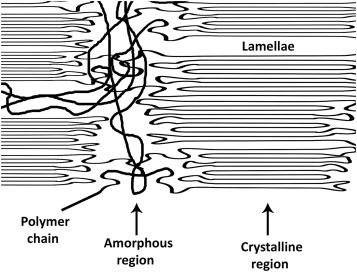
\includegraphics[width=0.4\textwidth]{fig/crystal-2.jpg}
    \caption{К определению кристалличности полимеров}
    \label{fig:crystal-2}
  \end{center}
  \vspace{-20pt}
  \vspace{1pt}
\end{wrapfigure}	

The two-phase model implied in Eq. (3.1) is only an approximation because
there can be a continuum of structures from large, defect-free single crystals to
the truly amorphous domains with liquid-like order. Because of the restrictions
imposed by long polymer chains, defects are invariably present in the crystal lattice,
and the polymer crystallites are small and disordered.\\
Conversely, the amorphous
domains possess some degree of positional and orientational correlations, and there
is experimental evidence for both rigid or ordered and soft or fluid amorphous phases\\
it may not always be possible to distinguish between the signatures
of the crystalline and amorphous phases. Nevertheless, a two-phase model with
an approximate crystalline phase and an amorphous phase, and sometimes an additional
ordered phase, mostly due to oriented amorphous domains, is often used.\\



\subsection{Влияние на макроскопические параметры}





	